\section{Computerarithmetik}

\subsection{Ganzzahlig}
\begin{tabular}{|p{3cm}|p{4.5cm}|p{4.5cm}|p{4.5cm}|}
\hline
Darstellung & Sign Magnitude & 1er Komplement & 2er Komplement\\
\hline
Zahlenbereich & $-(2^{n-1}-1)$ bis $+(2^{n-1}-1)$ & $-(2^{n-1}-1)$ bis +$(2^{n-1}-1)$ & $-2^{n-1}$ bis +$(2^{n-1}-1)$\\
\hline
Vorteil & Vorzeichen kann einfach durch Vorzeichenbit festgestellt werden. & Vorzeichen kann einfach durch MSB festgestellt werden. Addition und Subtraktion einfach realisierbar. & Vorzeichen kann einfach durch MSB festgestellt werden. Addition und Subtratkion einfach realisierbar \\ 
\hline
Nachteil & Positive und negative Null. Addition/Subtraktion kompliziert. & Positive und negative Null. & Keine Nachteile\\
\hline
Beispiel +5 & 0101 & 0101 & 0101 \\
Beispiel -5 & 1101 & 1010 & 1011 \\
\hline
\end{tabular}
\subsubsection{Addition/Subtraction}
Wird direkt mit Arithmetic Logic Unit (ALU) durchgef"uhrt.
\subsubsection{Multiplikation}
Mit ALU, Schieberegister und Ablaufsteuerung. Berechnungszeit nimmt linear mit Wortbreite zu. Schiebe Zahl x um n Stellen nach \textbf{links} $\rightarrow$ Multiplikation von x mit der n-ten Zweierpotenz. \\
Implementation Algorithmisch: Langsam, wenig Aufwand
\begin{itemize}
\item Mikroprogramm
\item Softwareemulation
\end{itemize}
Implementation Hardware: Schnell, viel Aufwand\\
\begin{itemize}
\item In vielen uC's drin, vor allem RISC (MSP430)
\item DSP ist HW-Multiplizierer ein Muss
\end{itemize}
\subsubsection{Division}
Mit Subtraktion, Schieberegister und Ablaufsteuerung. 
Implementation wie oben, jedoch HW-Dividierer eher selten, da Operation eher selten. Schiebe Zahl x um n Stellen nach \textbf{rechts} $\rightarrow$ Division von x durch die n-ten Zweierpotenz.\\
\subsubsection{Addierer}
Wichtigste arithmetische Funktion, n-Addierer werden auf 1-Bit Addierer zur"uck gef"uhrt. \\ \\
\textbf{Halbaddierer:}\\ \\
\begin{minipage}{0.5\textwidth}
	\centering
	\begin{tabular}{|c | c | c | c |}
	\hline
	A & B & Sum & Carry\\
	\hline
	0 & 0 & 0 & 0\\
	\hline
	0 & 1 & 1 & 0\\
	\hline
	1 & 0 & 1 & 0\\
	\hline
	1 & 1 & 0 & 1\\
	\hline
	\end{tabular}
\end{minipage}
\begin{minipage}{0.9\textwidth}
	\centering
	\begin{flushleft}
	{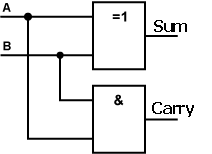
\includegraphics[width=0.3\textwidth]{images/Arithmetik/halbaddierer.png}}
	\label{Fig: Halbaddierer}
	\end{flushleft}
\end{minipage}\\ \\

\newpage
\textbf{Volladierer:}\\ \\

\begin{minipage}{0.5\textwidth}
	\begin{tabular}{|c | c | c | c | c |}
	\hline
	A & B & Carry In & Sum & Carry Out\\
	\hline
	0 & 0 & 0 & 0 & 0\\
	\hline
	0 & 0 & 1 & 1 & 0\\
	\hline
	0 & 1 & 0 & 1 & 0\\
	\hline
	0 & 1 & 1 & 0 & 1\\
	\hline
	1 & 0 & 0 & 1 & 0\\
	\hline
	1 & 0 & 1 & 0 & 1\\
	\hline
	1 & 1 & 0 & 0 & 1\\
	\hline
	1 & 1 & 1 & 1 & 1\\
	\hline
	\end{tabular}
\end{minipage}
\begin{minipage}{0.9\textwidth}
	\begin{flushleft}
	{
\includegraphics[width=0.5\textwidth]{images/Arithmetik/volladdierer.png}}
	\label{Fig: Volladdierer}
	\end{flushleft}
\end{minipage}\\ \\

\textbf{Subtrahierer:}\\
Subtraktion = Addition einer negativen Zahl (Bits invertieren plus 1)\\

\textbf{S"attigungsarithmetik:}\\
Es gibt keinen Over- bzw. Underflow, sondern der h"ochste bzw. niedrigste Wert wird einfach bei behalten.\\
\subsection{Fixpunkt}
Dezimalpunkt sitzt an fester Stelle, die unteren Dezimalstellen werden als negative Zweierpotenzen interpretiert. \\
Fixed point ist einfach zu implementieren. 
\subsection{Gleitkomma}
\begin{equation}
(-1)^S\cdot M \cdot B^E
\end{equation}
S = Vorzeichen (float: 1 bit double:1 bit)\\
M = Mantisse (float:23 bit double: 52 bit)\\
B = Basis \\
E = Exponent (float:8 bit double:11 bit)\\

Floating Point Unit (FPU): HW-Implementation zur Berechnung von Floating Point Zahlen. Kann auch Wurzeln, Trigo etc.\\

\subsubsection{Newton-Raphson}
Um eine unäre Funktion wie $sin(x)$ zu berechnen, kann man die Taylorreihe verwenden $sin(x) = x - \frac{x^3}{3!} + \frac{x^5}{5!} - \frac{x^7}{7!}$. Die Koeffizienten k"onnten gespeichert werden, jedoch ist die Konvergenz trotz dieser Vereinfachung langsam. 
Eine Methode, welche schneller konvergiert ist das Newton-Raphson Verfahren: 
\begin{equation}
y_{k+1} = y_k - \frac{f(y_k)}{\frac{\partial}{\partial y}f(y_k)}
\end{equation}
Zur Berechnung einer Reziproken $g(x)=\frac{1}{x}=y$ ergibt sich folgende Formel: 
\begin{equation}
y_{k+1} = y_k\cdot (2-x\cdot y_k)
\end{equation}
Wobei $x$ die Zahl aus dem Reziprokwert ist und $y_k$ ein vern"unftiger Anfangswert ist. \\

Somit kann auch die Quadratwurzel berechnet werden und zwar via: $\frac{1}{\sqrt{x}} \cdot x = \sqrt{x}$\\
Wobei der Bruch $\frac{1}{\sqrt{x}}$ wie folgt berechnet werden kann:
\begin{equation}
y_{k+1} = 0.5y_k\cdot (3-x\cdot y_k^2)
\end{equation}
Das Newton Verfahren konvergiert quadratisch, d.h mit jedem Durchlauf kann die Genauigkeit verdoppelt werden.\\
Ablauf Addition/Subtraktion/Multiplikation/Division siehe Folien.\\
Ausserdem siehe dort auch Infos zu Beispielarchitekturen.

